\documentclass[12pt]{article}

% 杂项宏包
\usepackage[colorlinks,linkcolor=blue]{hyperref}  % 超链接
\usepackage{amsmath}
\usepackage{amssymb}
\usepackage{multicol}
\usepackage{indentfirst}
\usepackage{algorithm}   % 代码块
\usepackage{algorithmicx}   % 代码块
\usepackage{algpseudocode}   % 代码块 
\usepackage{graphicx}  % 图片
\usepackage{subfigure}  % 并排图像
\usepackage{fontspec}
%\usepackage{parskip}
\usepackage[]{caption2}  % 去掉图表的冒号
\renewcommand{\captionlabeldelim}{}  % 去掉图表的冒号
\usepackage{booktabs} % 三线表
\usepackage{pdfpages}  % 直接插入pdf页面
% \setlength{\parindent}{2em}

% 字体设置
\usepackage{xeCJK}
%%%%%%%%%%% CJK下设置中文字体 %%%%%%%%%%%%%
\setCJKfamilyfont{song}{SimSun.ttf}
\newcommand{\song}{\CJKfamily{song}}
\setCJKfamilyfont{kai}{simkai.ttf}
\newcommand{\kai}{\CJKfamily{kai}}
\setCJKfamilyfont{fang}{simfang.ttf}
\newcommand{\fang}{\CJKfamily{fang}}
\setCJKfamilyfont{hei}{simhei.ttf}
\newcommand{\hei}{\CJKfamily{hei}}
\setCJKfamilyfont{li}{SIMLI.TTF}
\newcommand{\li}{\CJKfamily{li}}
\setmainfont{times.ttf}  % 英文字体
\setsansfont{Source Sans Pro}
\setmonofont{simkai.ttf}
\setCJKmainfont{SimSun.ttf}  % 中文字体
\setCJKsansfont{simhei.ttf}
\setCJKmonofont{simkai.ttf}


\usepackage{gbt7714}  % 国标参考文献
\renewcommand\refname{\hei \sihao 参考文献}

% 页面布局设置
\usepackage{geometry}
\geometry{a4paper, scale=0.8}  % 页面边距
% \setlength{\parskip}{1.15em}  % 段落之间空 0.5 行


% 其他设置
%%%%%%%%%%%  设置字体大小 %%%%%%%%%%%%%
\newcommand{\chuhao}{\fontsize{42pt}{\baselineskip}\selectfont}   %%%初号字体
\newcommand{\xiaochuhao}{\fontsize{36pt}{\baselineskip}\selectfont}    %%%小初号字体
\newcommand{\yihao}{\fontsize{28pt}{\baselineskip}\selectfont}   %%%一号字体,以此类推
\newcommand{\erhao}{\fontsize{21pt}{\baselineskip}\selectfont}
\newcommand{\xiaoerhao}{\fontsize{18pt}{\baselineskip}\selectfont}
\newcommand{\sanhao}{\fontsize{15.75pt}{\baselineskip}\selectfont}
\newcommand{\sihao}{\fontsize{14pt}{\baselineskip}\selectfont}
\newcommand{\xiaosihao}{\fontsize{12pt}{\baselineskip}\selectfont}
\newcommand{\wuhao}{\fontsize{10.5pt}{\baselineskip}\selectfont}
\newcommand{\xiaowuhao}{\fontsize{9pt}{\baselineskip}\selectfont}
\newcommand{\liuhao}{\fontsize{7.875pt}{\baselineskip}\selectfont}
\newcommand{\qihao}{\fontsize{5.25pt}{\baselineskip}\selectfont}

%%%% 设置 section 属性 %%%%
\makeatletter  
\renewcommand\section{\@startsection{section}{1}{\z@}%
	{-1.5ex \@plus -.5ex \@minus -.2ex}%
	{.5ex \@plus .1ex}%
	{\normalfont\sihao\fang}}  %%这边要是不想要宋体三号字,可以把song改成之前定义的字体和字号。
	%{\normalfont\sihao\CJKfamily{fs}}}  %%比如改成仿宋四号,前面定义好了,后面只需要改几个字母就可以了。
\makeatother
%%%% 设置 subsection 属性 %%%%
\makeatletter
\renewcommand\subsection{\@startsection{subsection}{1}{\z@}%
	{-1.25ex \@plus -.5ex \@minus -.2ex}%
	{.4ex \@plus .1ex}%
	{\normalfont\wuhao\hei}}
\makeatother
%%%% 设置 subsubsection 属性 %%%%
\makeatletter
\renewcommand\subsubsection{\@startsection{subsubsection}{1}{\z@}%
	{-1ex \@plus -.5ex \@minus -.2ex}%
	{.3ex \@plus .1ex}%
	{\normalfont\wuhao\song}}
\makeatother
% 章节从 0 开始
\setcounter{section}{-1}

% 算法标题设置
\floatname{algorithm}{\xiaowuhao 算法}  
\renewcommand{\algorithmicrequire}{\textbf{输入:}}  
\renewcommand{\algorithmicensure}{\textbf{输出:}} 

\renewcommand{\figurename}{\xiaowuhao \hei 图}
\renewcommand{\tablename}{\xiaowuhao \hei 表}

  % 导入配置文件

\newcommand\titleofdoc{} % 文档标题
\newcommand\GroupName{} % 小组名

\usepackage{fancyhdr}
\pagestyle{fancy}
\fancyhf{}
\fancyhead[C]{\small 中国石油大学(华东)}

\setcounter{section}{0}


% 正文
%%%%%%%%%%%%%%%%%%%%%%%%%%%%%%%%%%%%%%%%%%%%%%%%%%%%%%%%%%%%%%%%%%%%%%%%%%%%%%%%%%%%%%%%%%%%%%%%%%%%%%%%%%%%%%%%%%%%%%%
\begin{document}
\begin{sloppypar}  % 两端对齐命令

 % \input{sections/cover.tex}  % 封面文件

 
    \begin{center}
        \erhao \sffamily 一款基于BiLSTM-CRF的英文选词填空机器作答应用设计

        \vspace{0.3cm}

        \xiaosihao \ttfamily 申\quad 鹏\quad 飞$^1$,作\quad 者$^2$

        \xiaowuhao (1.智能科学与技术2102 2115040110;2.作者详细单位,省市 邮编)
    \end{center}

    \xiaowuhao{
        \noindent \sffamily 摘要: \normalfont 在英文选词填空题目中,文章中的句子空缺通常具有多个选项。
        条件随机场的前向算法能够计算出填入各选项后的句子的“前向分数”,从而判断出最佳的选项。
        由百度研究院提出的双向长短时记忆-条件随机场模型是Transformer时代之前最成熟的序列标注模型之一,该网络通过结合双向长短时记忆网络和条件随机场,有较强的结构表示能力。
        本次报告将详细介绍基于该模型的选词填空机器答题应用的设计原理和表现效果。

        \noindent \sffamily 关键词:\normalfont 完形填空;机器答题;双向长短时记忆网络;条件随机场
       }

       \begin{center}
        \sihao Machine Answering For English Fill-In-The-Blank Word Selection Quizzes Based On BiLSTM-CRF Segmentation

        \vspace{0.3cm}

        \xiaosihao Shen pengfei$^1$,NAME Name-name$^2$

        \xiaowuhao (1. Artifical Intelligence Science and Engineering 2102 2115040110; 2. Department, City, City Zip Code, China)

    \end{center}
    \xiaowuhao{
        \noindent \textbf{Abstract: }In English Fill-in-the-Blank word selection quizzes, there are multiple options for a blank. 
        The forward algorithm of conditional random field can `predict' the option with the highest forward score, so as to choose the most likely answer.
        The bidirectional long short-term memory - conditional random field model was one of the most mature sequence annotation models before the Transformer era, which includes a conditional random field layer.
        This paper will introduce in detail the design and performance of the fill-in-the-blank word selection machine based on this model.

        \noindent \textbf{Keywords: }Fill-in-the-Blank; Machine Answering; Bidirectional Long Short-Term Memory; Conditional Random Field
       }

  % 标题及摘要文件

 \vspace{0.5cm}  % 分隔 0.5cm
 

 \section{引言}  % 第一个section的标题(一般为引言,此处不分栏,因为根据 word 模板来看,这一行似乎是单独的,但是内容又是要分栏的,所以把第一个section的标题和内容分开了)
 	\begin{multicols*}{2}  % 正文开始分栏
 	
    “词性标注”是自然语言处理的经典任务之一,AI能根据输入的句子推测出对应词性序列。
目前,主流的模型网络都结合了条件随机场(CRF)层。
许多学者和工程师基于CRF的前向算法提出了基于序列标注的文本生成应用,如RNN的诗歌生成应用等。
在生成式算法中,模型会将“前向分数”最大的句子作为最终的生成结果。

此外,关于英文选词填空机器答题的应用,一些学者已经提出了一些比较独特的方法,如来自Google团队的MaskGAN网络。
Transformer框架问世后,互联网上出现了大量的基于BERT的中英文选词填空应用,如Unmask等。
这些网络较BiLSTM-CRF各有优缺点。
\subsection{OCR的作用}
123123123213123123引言内容。引言作为论文的开场白,应以简短的篇幅介绍论文的写作背景和目的,以及相关领域内前人所做的工作和研究概况,说明本研究与前人工作的关系,目前研究的热点、存在的问题及作者工作的意义。1、开门见山,不绕圈子。避免大篇幅地讲述历史渊源和立题研究过程。2、言简意赅,突出重点。不应过多叙述同行熟知的及教科书中的常识性内容,确有必要提及他人的研究成果和基本原理时,只需以引用参考文献的形势标出即可。在引言中提示本文的工作和观点时,意思应明确,语言应简练。3、引言的内容不要与摘要雷同,也不是摘要的注释。4、引言要简短,最好不要分段论述,不要插图、列表和数学公式。  % 第一个section的内容,接上面的标题
    
    \section{量的书写规则}
正文内容。正文、图表中的变量都要用斜体字母,对于矢量和张量使用黑斜体,只有pH采用正体;使用新标准规定的符号\cite{simonyan2014very};量的符号为单个拉丁字母或希腊字母;不能把量符号作为纯数使用;不能把化学符号作为量符号使用,代表物质的符号表示成右下标,具体物质的符号及其状态等置于与主符号齐线的圆括号中。

注意区分量的下标字母的正斜体:凡量符号和代表变动性数字及坐标轴的字母作下标,采用斜体字母。

正文中引用参考文献的标注方法,在引用处对引用的文献,按它们在论著中出现的先后用阿拉伯数字连续排序,将序号置于方括号内,并视具体情况把序号作为上角标或作为语句的组成部分。
\subsection{单位的书写规则}
正文内容。单位符号无例外的采用正体字母。注意区分单位符号的大小写:一般单位符号为小写体,来源于人名的单位符号首字母大写。体积单位升的符号为大写L。
\subsubsection{表格的规范化}
正文内容。表格的设计应该科学、明确、简洁,具有自明性。表格应采用三线表,项目栏不宜过繁,小表宽度小于7.5 cm,大表宽度为12~15cm 。表必须有中英文表序、表题。表中顶线与栏目线之间的部分叫项目栏,底线与栏目线之间的部分叫表身。表身中数字一般不带单位,百分数也不带百分号,应把单位符号和百分号等归并在栏目中。如果表中栏目中单位均相同,则可把共同的单位提出来标示在表格顶线上方的右端(不加“单位”二字)。表身中同一栏各行的数值应以个位(或小数点),且有效位数相同。上下左右相邻栏内的文字或数字相同时,应重复写出。

\begin{table}[H]
	\xiaowuhao
	\centering
	\caption{\label{tab11} \xiaowuhao \hei 表题}
	\begin{tabular}{llll}
		\toprule
		Model                 & SMO+DNN & PCA+DNN & DNN   \\
		\midrule
		Accuracy              & 0.994   & 0.938   & 0.914 \\
		Precision             & 0.995   & 0.934   & 0.891 \\
		Recall                & 0.995   & 0.918   & 0.882 \\
		\bottomrule
	\end{tabular}
\end{table}  % 第二个section(标题加内容)
    
    \section{图}
正文内容。插图尽可能不用彩色图。小图宽度小于7.5 cm,大图宽度为12~15cm 。图必须有中英文图序、图题。函数图只在靠近坐标线处残留一小段标值短线,其余部分省略。加注坐标所代表的量及单位(如t/s)。标值排印在坐标外侧,紧靠标值短线的地方;标值的有效数字为3位。图中量的意义要在正文中加以解释。若有图注,靠近放在图下部,图序、图题的上方。

\begin{figure}[H]
	\centering
	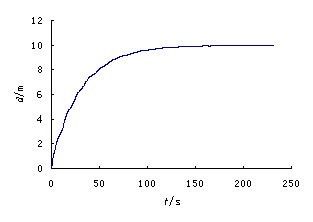
\includegraphics[width=3in]{sections/figs/template.png}
	\caption{\label{fig1111} \xiaowuhao \hei 图题}
\end{figure}

\section{数学符号和数学式的编排规范}
正文内容。变量、变动附标及函数用斜体字母表示。点、线段及弧用斜体字母表示。在特定场合中视为常数的参数也用斜体字母表示。对具有特殊定义的函数和值不变的数学常数用正体字母表示。具有特殊定义的算子也用正体字母表示。矩阵符号用大写的黑斜体字母表示,矩阵元素用白斜体字母表示。

公式及公式中的符号说明尽量接排以节省版面。把带有复杂上角标的指数函数$e^t$ 写成$\exp{t}$ 。公式的主体应排在同一水平线上;繁分式的主辅线要分清。长公式在运算符号后回行;长分式转行时,先将分母写成负幂指数的形式,然后转行;矩阵和行列式不能转行。矩阵元素包含式子时,每一列应以中心线上下对齐,行要左右排齐;元素为单个字母或数字时,每列应使正负号对齐。对角矩阵中对角元素所在的列应明显区分,不能上下重叠。

简单的和常识性的运算公式和推导过程不要列写。

\begin{equation}
	\label{equ333}
	\begin{split}
		\left \{
		\begin{array}{ll}
			O_i = X &i=1 \\
			O_i = f_i(Z_i) & i>1 \\
			Z_i = g_i(O_{i-1}, W_i)
		\end{array}
		\right.
	\end{split}
\end{equation}

\begin{equation}
	\label{equa555}
	F_D = \beta \star (1-A) + (1-\beta) \star \frac{S}{D}
\end{equation}

\section{结束语}
正文内容。结论不应是正文中各段小结的简单重复,它应以正文中的实验或考察得到的现象、数据的阐述分析为依据,完整、准确、简洁地指出以下内容:1)由对研究对象进行考察或实验得到的结果所揭示的原理及其普遍性;2)研究中有无发现例外或本论文尚难以解释和解决的问题;3)与先前发表过的研究工作的异同;4)本文在理论上和实用上的意义及价值;5)进一步深入研究本课题的建议。  % 

    % ...后续section
    
    
    % 参考文献
   %  \bibliographystyle{plain}  % 参考文献的格式
   \vspace{0.5cm}
   	\nocite{*}
    \bibliography{sections/refs.bib}  % 参考文献bib文件
    \end{multicols*}
 
 
\end{sloppypar}
\end{document}

%%%%%%%%%%%%%%%%%%%%%%%%%%%%%%%%%%%%%%%%%%%%%%%%%%%%%%%%%%%%%%%%%%%%%%%%%%%%%%%%%%%%%%%%%%%%%%%%%%%%%%%%%%%%%%%%%%%%%%%%%%%%%%%%%%%%%%%%%%%%%%%%%%%%%%